\section{Visualization}

The Generalized Orthogonal Vectors Generator and Visualizer package provides various visualization options for the generated vectors. This section describes the visualization techniques used by the package.

\subsection{3D Visualization}

The 3D visualization shows the vectors in three-dimensional space. It uses Matplotlib's 3D plotting capabilities to create a 3D plot with the following features:

\begin{itemize}
    \item The origin point is shown as a black dot.
    \item The vectors are shown as arrows from the origin point.
    \item Each vector is assigned a different color for easy identification.
    \item The plot includes a legend identifying each vector.
    \item The plot includes labels for the X, Y, and Z axes.
    \item The plot includes a title, which can be customized.
\end{itemize}

The 3D visualization provides a complete view of the vectors in three-dimensional space, allowing for a better understanding of their spatial relationships.

\begin{figure}[H]
    \centering
    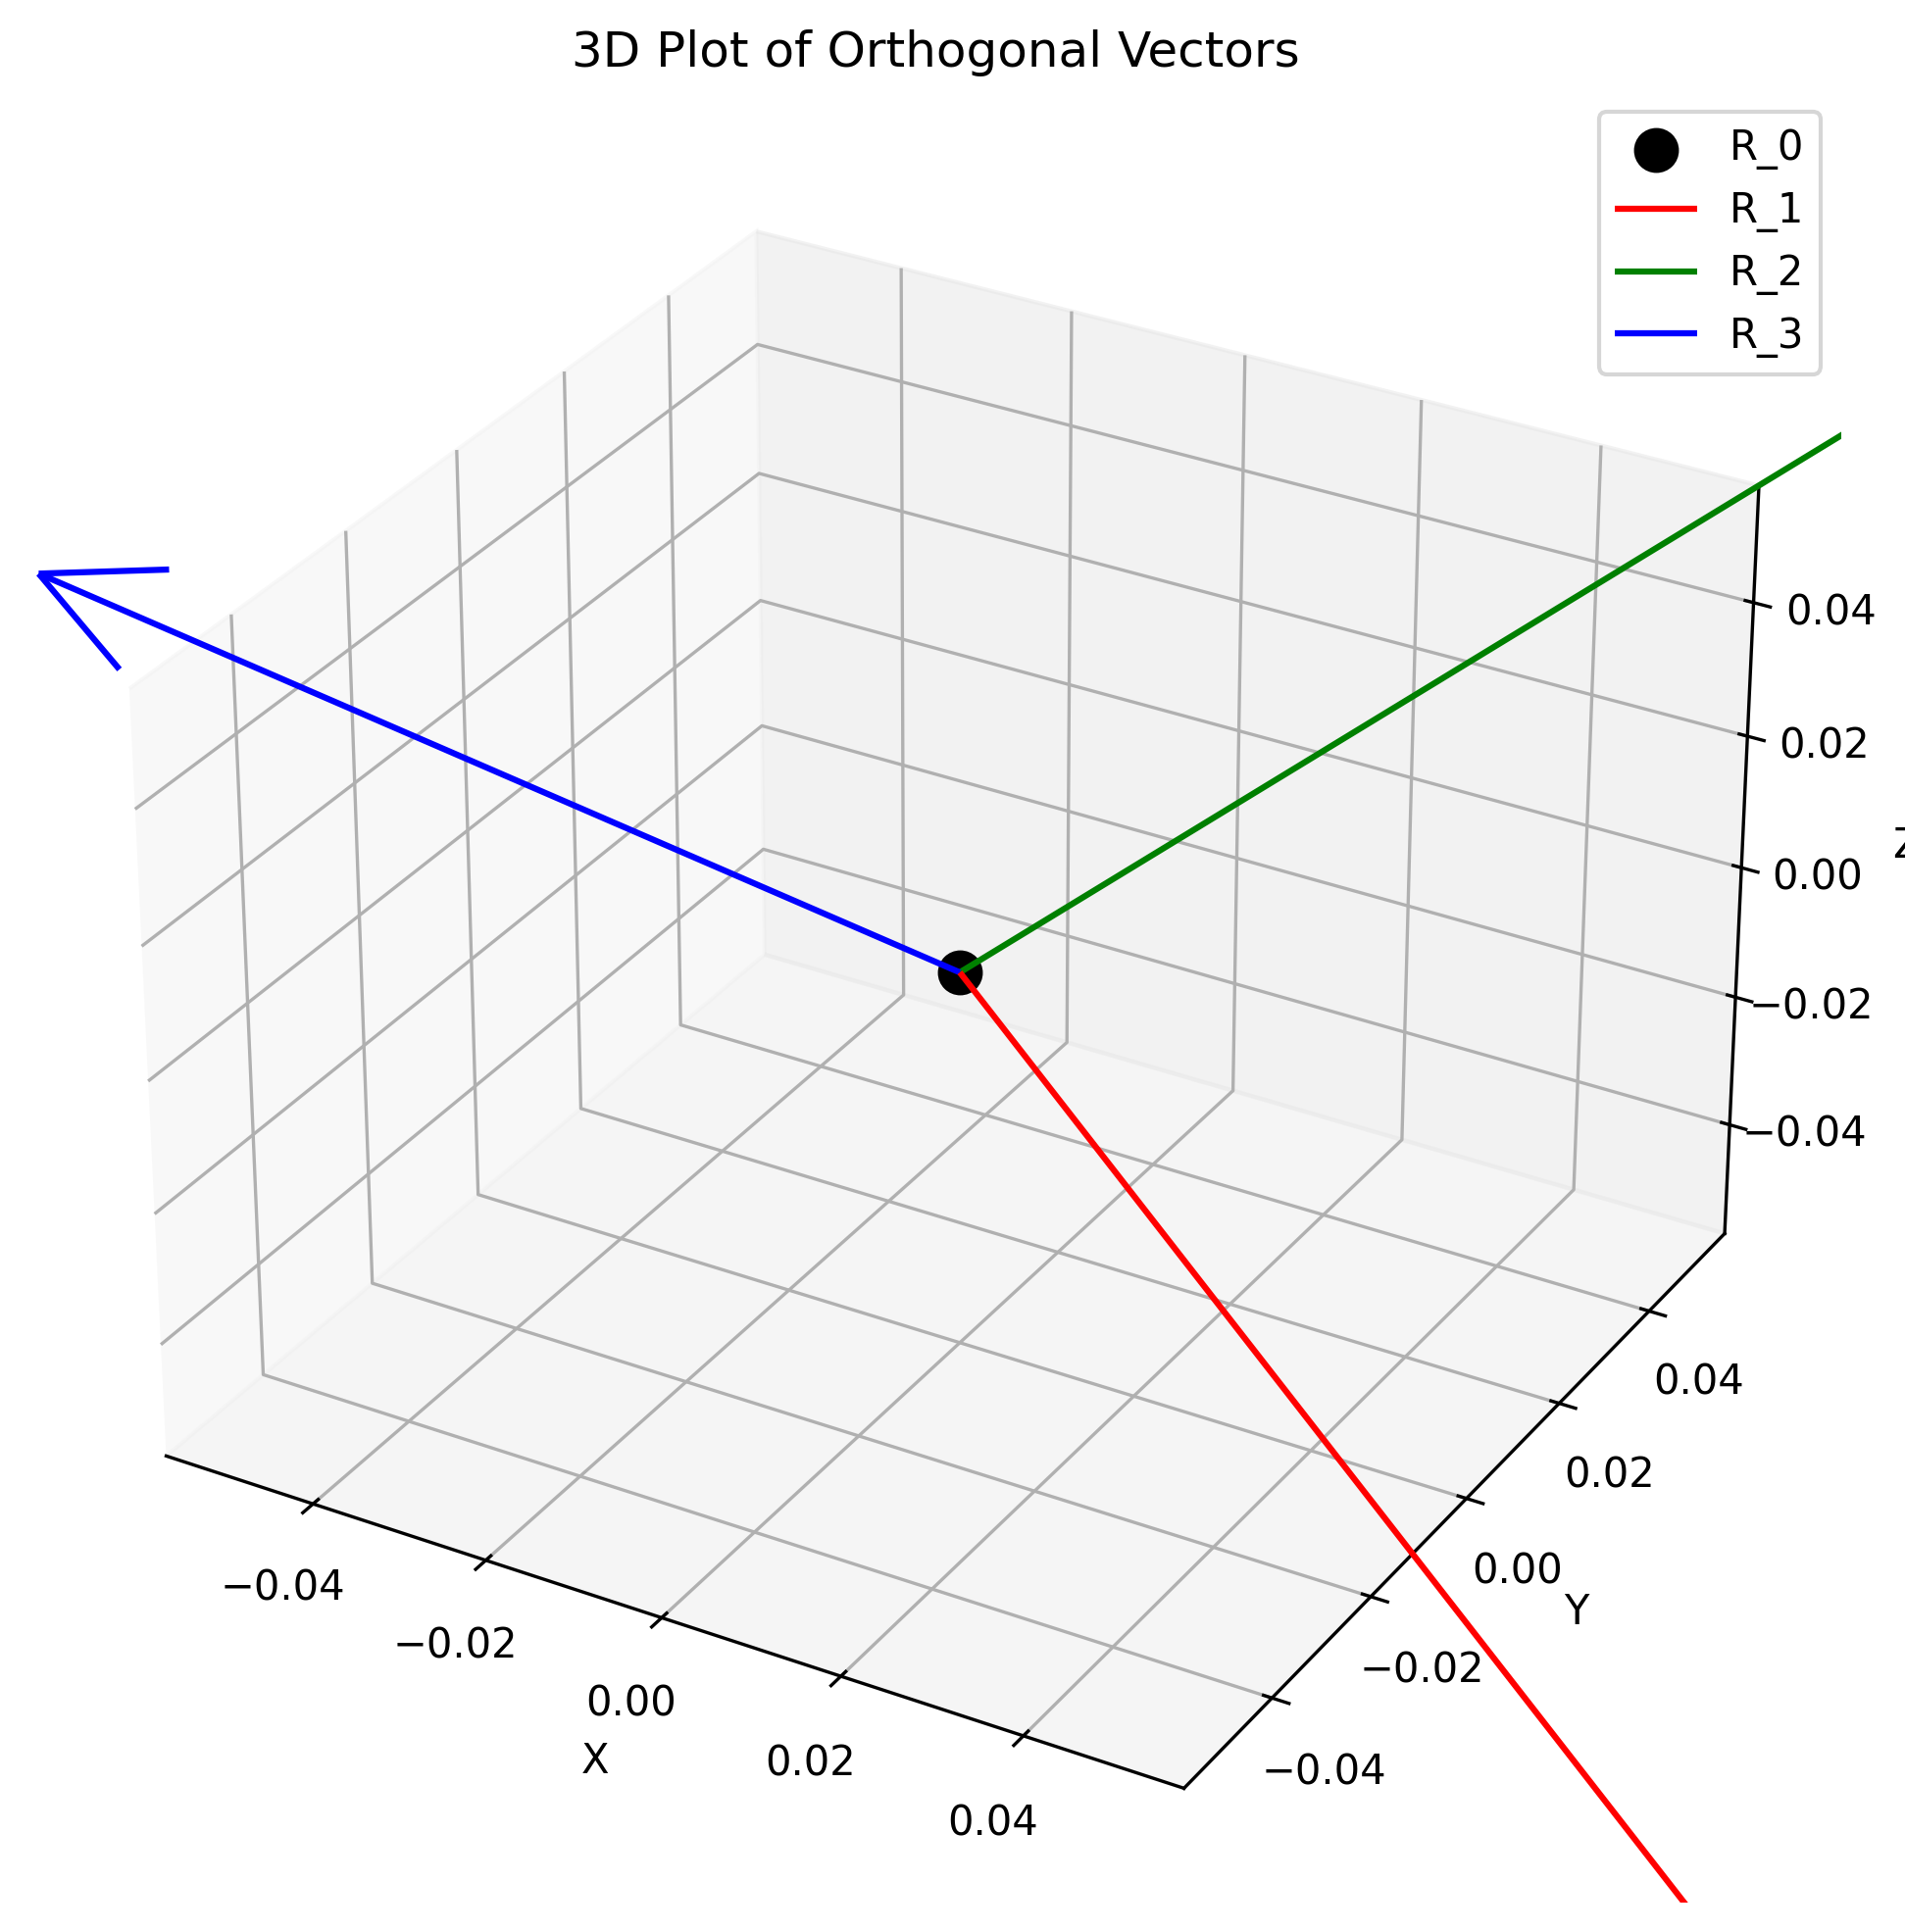
\includegraphics[width=0.8\textwidth]{figures/3d_plot.png}
    \caption{Example of 3D visualization}
    \label{fig:vis_3d_plot}
\end{figure}

\subsection{2D Projections}

The 2D visualization shows projections of the vectors onto various planes. It creates four subplots showing the following projections:

\begin{itemize}
    \item XY Plane: Shows the projection of the vectors onto the XY plane (Z=0).
    \item XZ Plane: Shows the projection of the vectors onto the XZ plane (Y=0).
    \item YZ Plane: Shows the projection of the vectors onto the YZ plane (X=0).
    \item R0 Plane: Shows the projection of the vectors onto the plane perpendicular to the vector from the global origin to $R_0$. This provides a clear view of the orthogonality of the vectors in the plane normal to the origin direction. The projection uses two orthogonal basis vectors in this plane:
        \begin{itemize}
            \item If $R_0$ is the origin (0,0,0), the basis vectors are derived from $R_1$ and $R_2$ after orthogonalization.
            \item Otherwise, the first basis vector is computed as the cross product of the normalized $R_0$ vector with either [1,0,0] or [0,1,0] (whichever is not parallel to $R_0$).
            \item The second basis vector is computed as the cross product of the normalized $R_0$ vector with the first basis vector, ensuring a perfectly orthogonal basis.
        \end{itemize}
\end{itemize}

Each subplot includes the following features:

\begin{itemize}
    \item The origin point is shown as a black dot.
    \item The vectors are shown as arrows from the origin point.
    \item Each vector is assigned a different color for easy identification.
    \item The subplot includes a legend identifying each vector.
    \item The subplot includes labels for the axes.
    \item The subplot includes a title indicating the plane of projection.
\end{itemize}

The 2D projections provide different perspectives on the vectors, allowing for a better understanding of their projections onto different planes.

\begin{figure}[H]
    \centering
    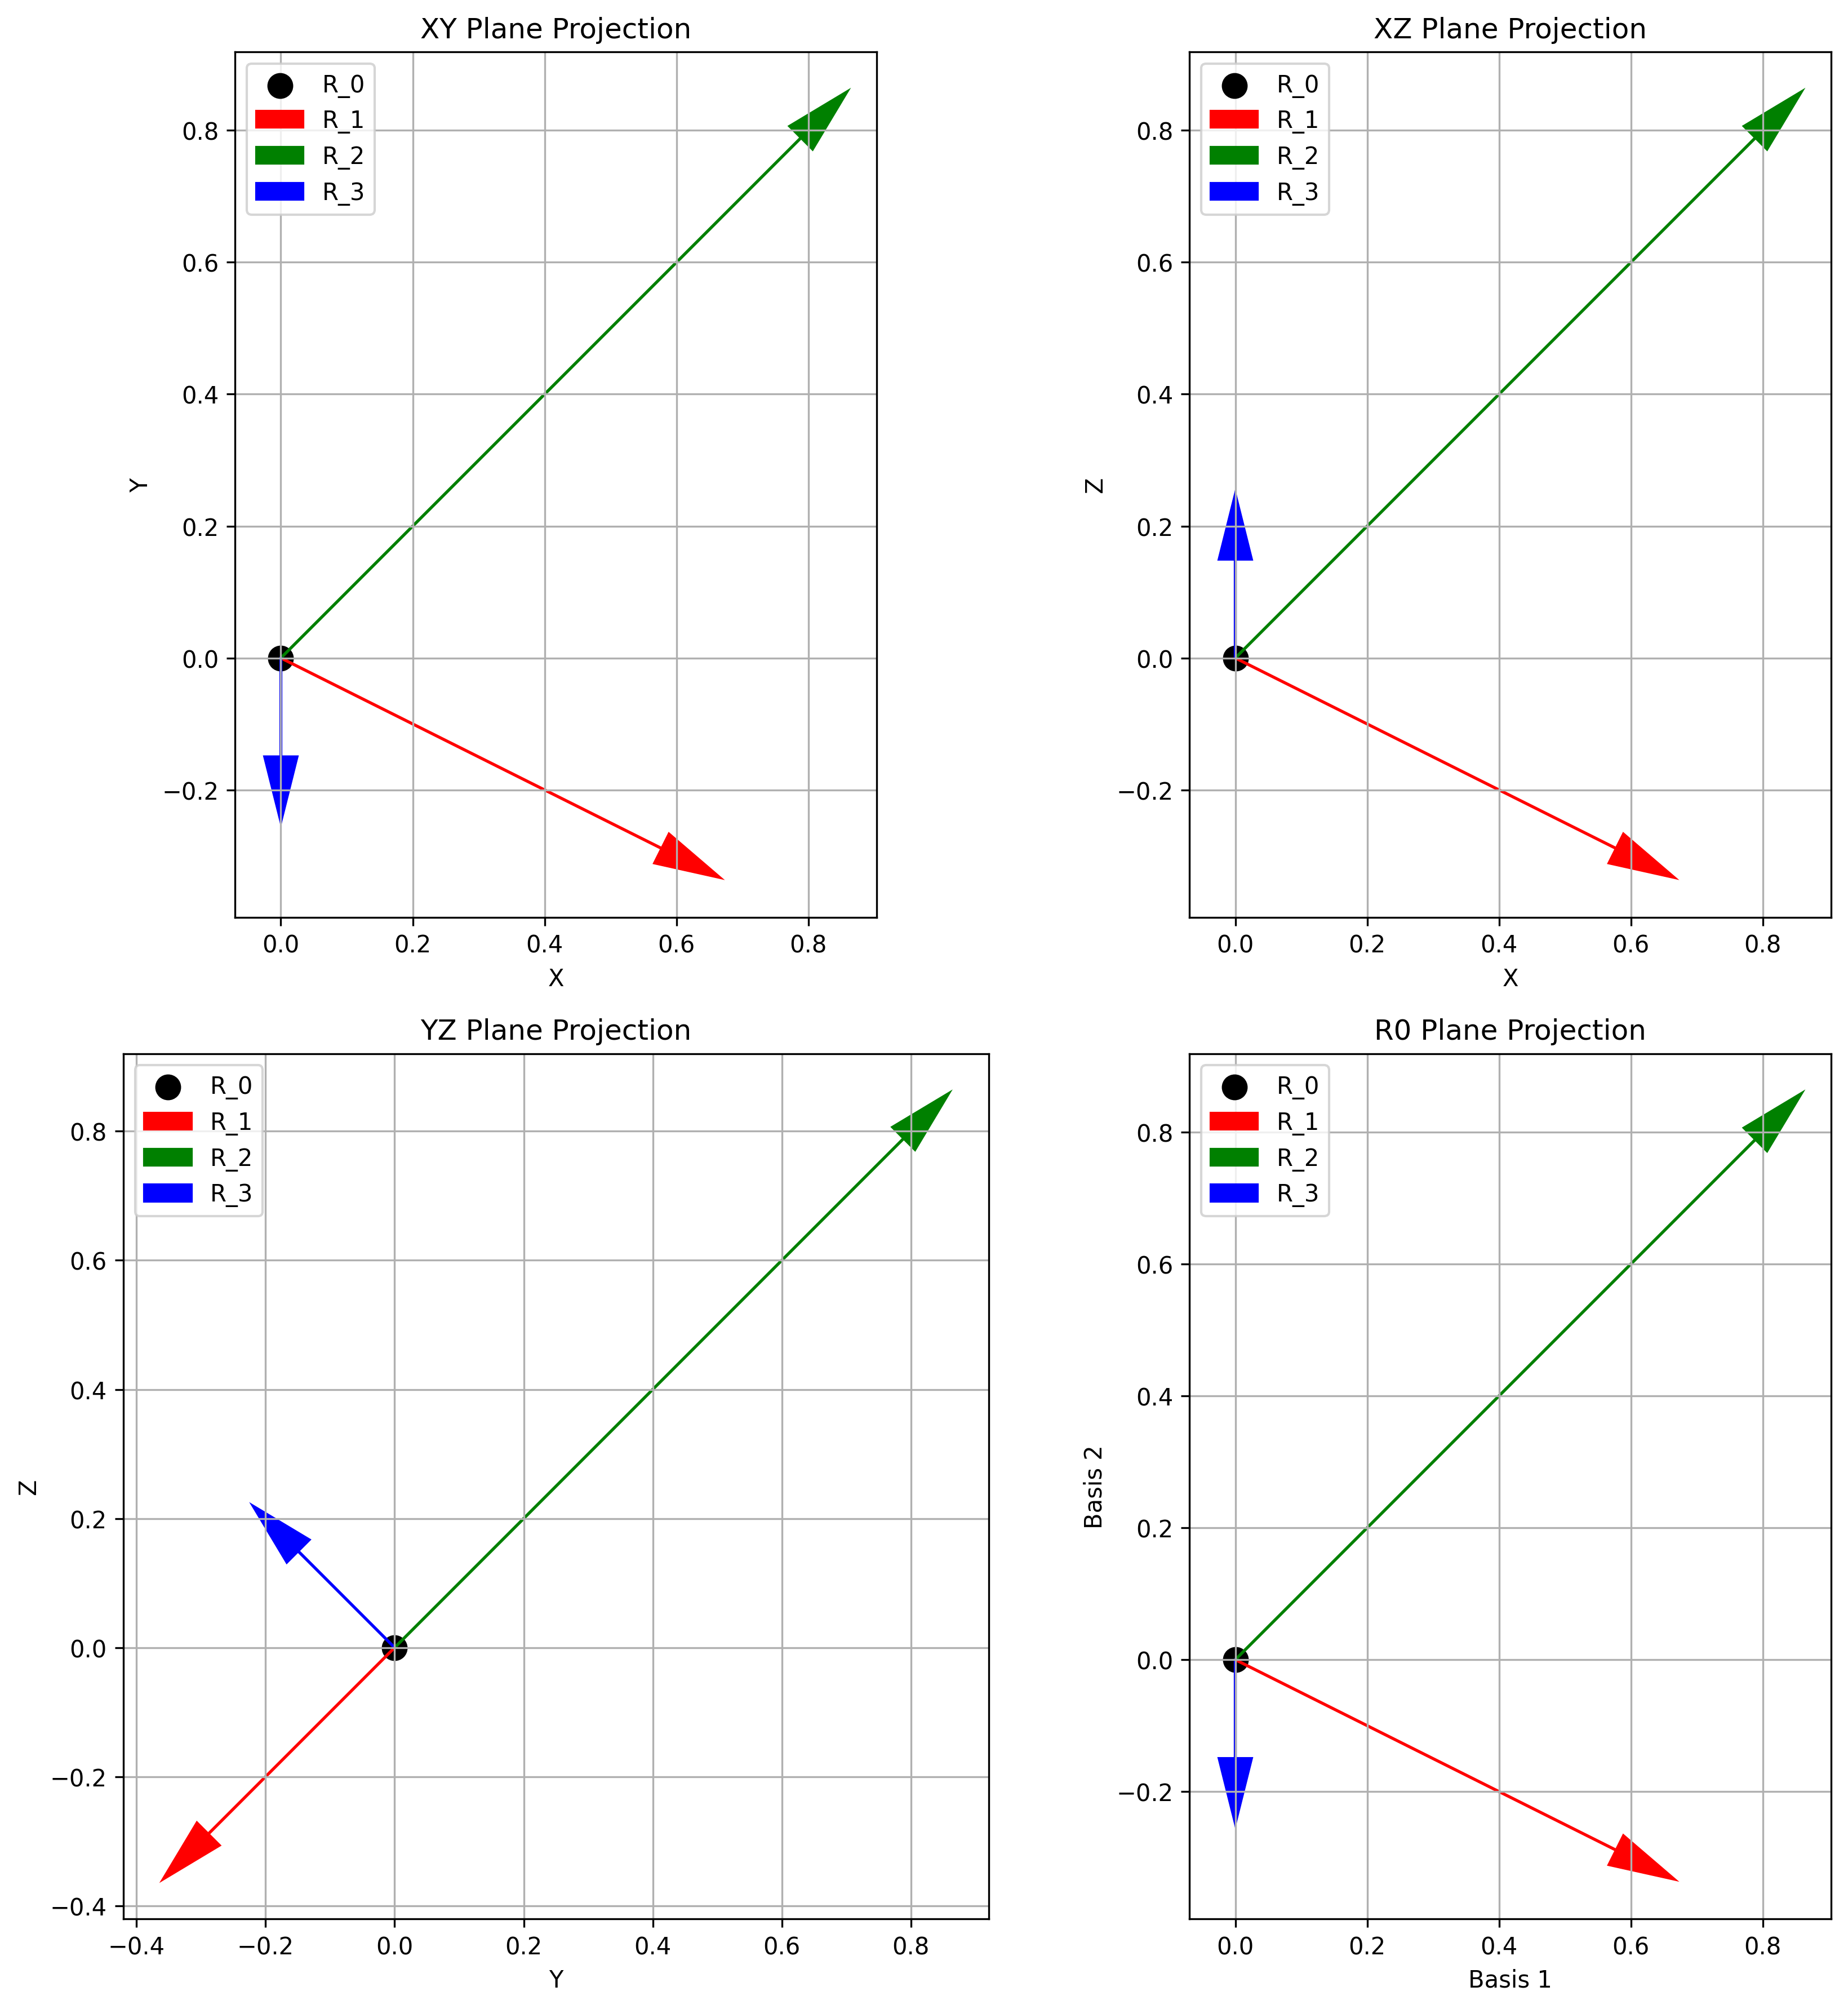
\includegraphics[width=0.8\textwidth]{figures/2d_projections.png}
    \caption{Example of 2D projections}
    \label{fig:vis_2d_projections}
\end{figure}

\subsection{Customization Options}

The visualization functions provide various customization options, including:

\begin{itemize}
    \item Plot title: The title of the plot can be customized.
    \item Show plot: The plot can be displayed interactively or not.
    \item Save path: The plot can be saved to a file instead of being displayed interactively.
\end{itemize}

These options can be specified directly when calling the visualization functions or through the \texttt{VectorConfig} class.

\subsection{R0 Plane Projections}

The package includes specialized scripts for generating R0 plane projections, which provide a clear view of the orthogonality of the vectors in the plane perpendicular to the origin direction:

\begin{itemize}
    \item \texttt{generate\_r0\_projections.py}: Generates R0 plane projections for various configurations with improved axis handling, symmetric axis limits, and better legend placement.
    \item \texttt{generate\_combined\_views.py}: Generates combined 3D and R0 plane projection figures, showing both perspectives side by side.
    \item \texttt{generate\_specific\_r0\_projections.py}: Generates R0 plane projections specifically for the three combined effect configurations (origins at $(0,0,0)$, $(1,1,1)$, and $(0,0,2)$).
\end{itemize}

These projections include the following enhancements:
\begin{itemize}
    \item Dynamic axis limit calculation with a 20\% margin to ensure all vector projections are visible
    \item Symmetric axis limits for better visual representation
    \item Improved grid for better readability
    \item Enhanced legend placement
\end{itemize}

\begin{figure}[H]
    \centering
    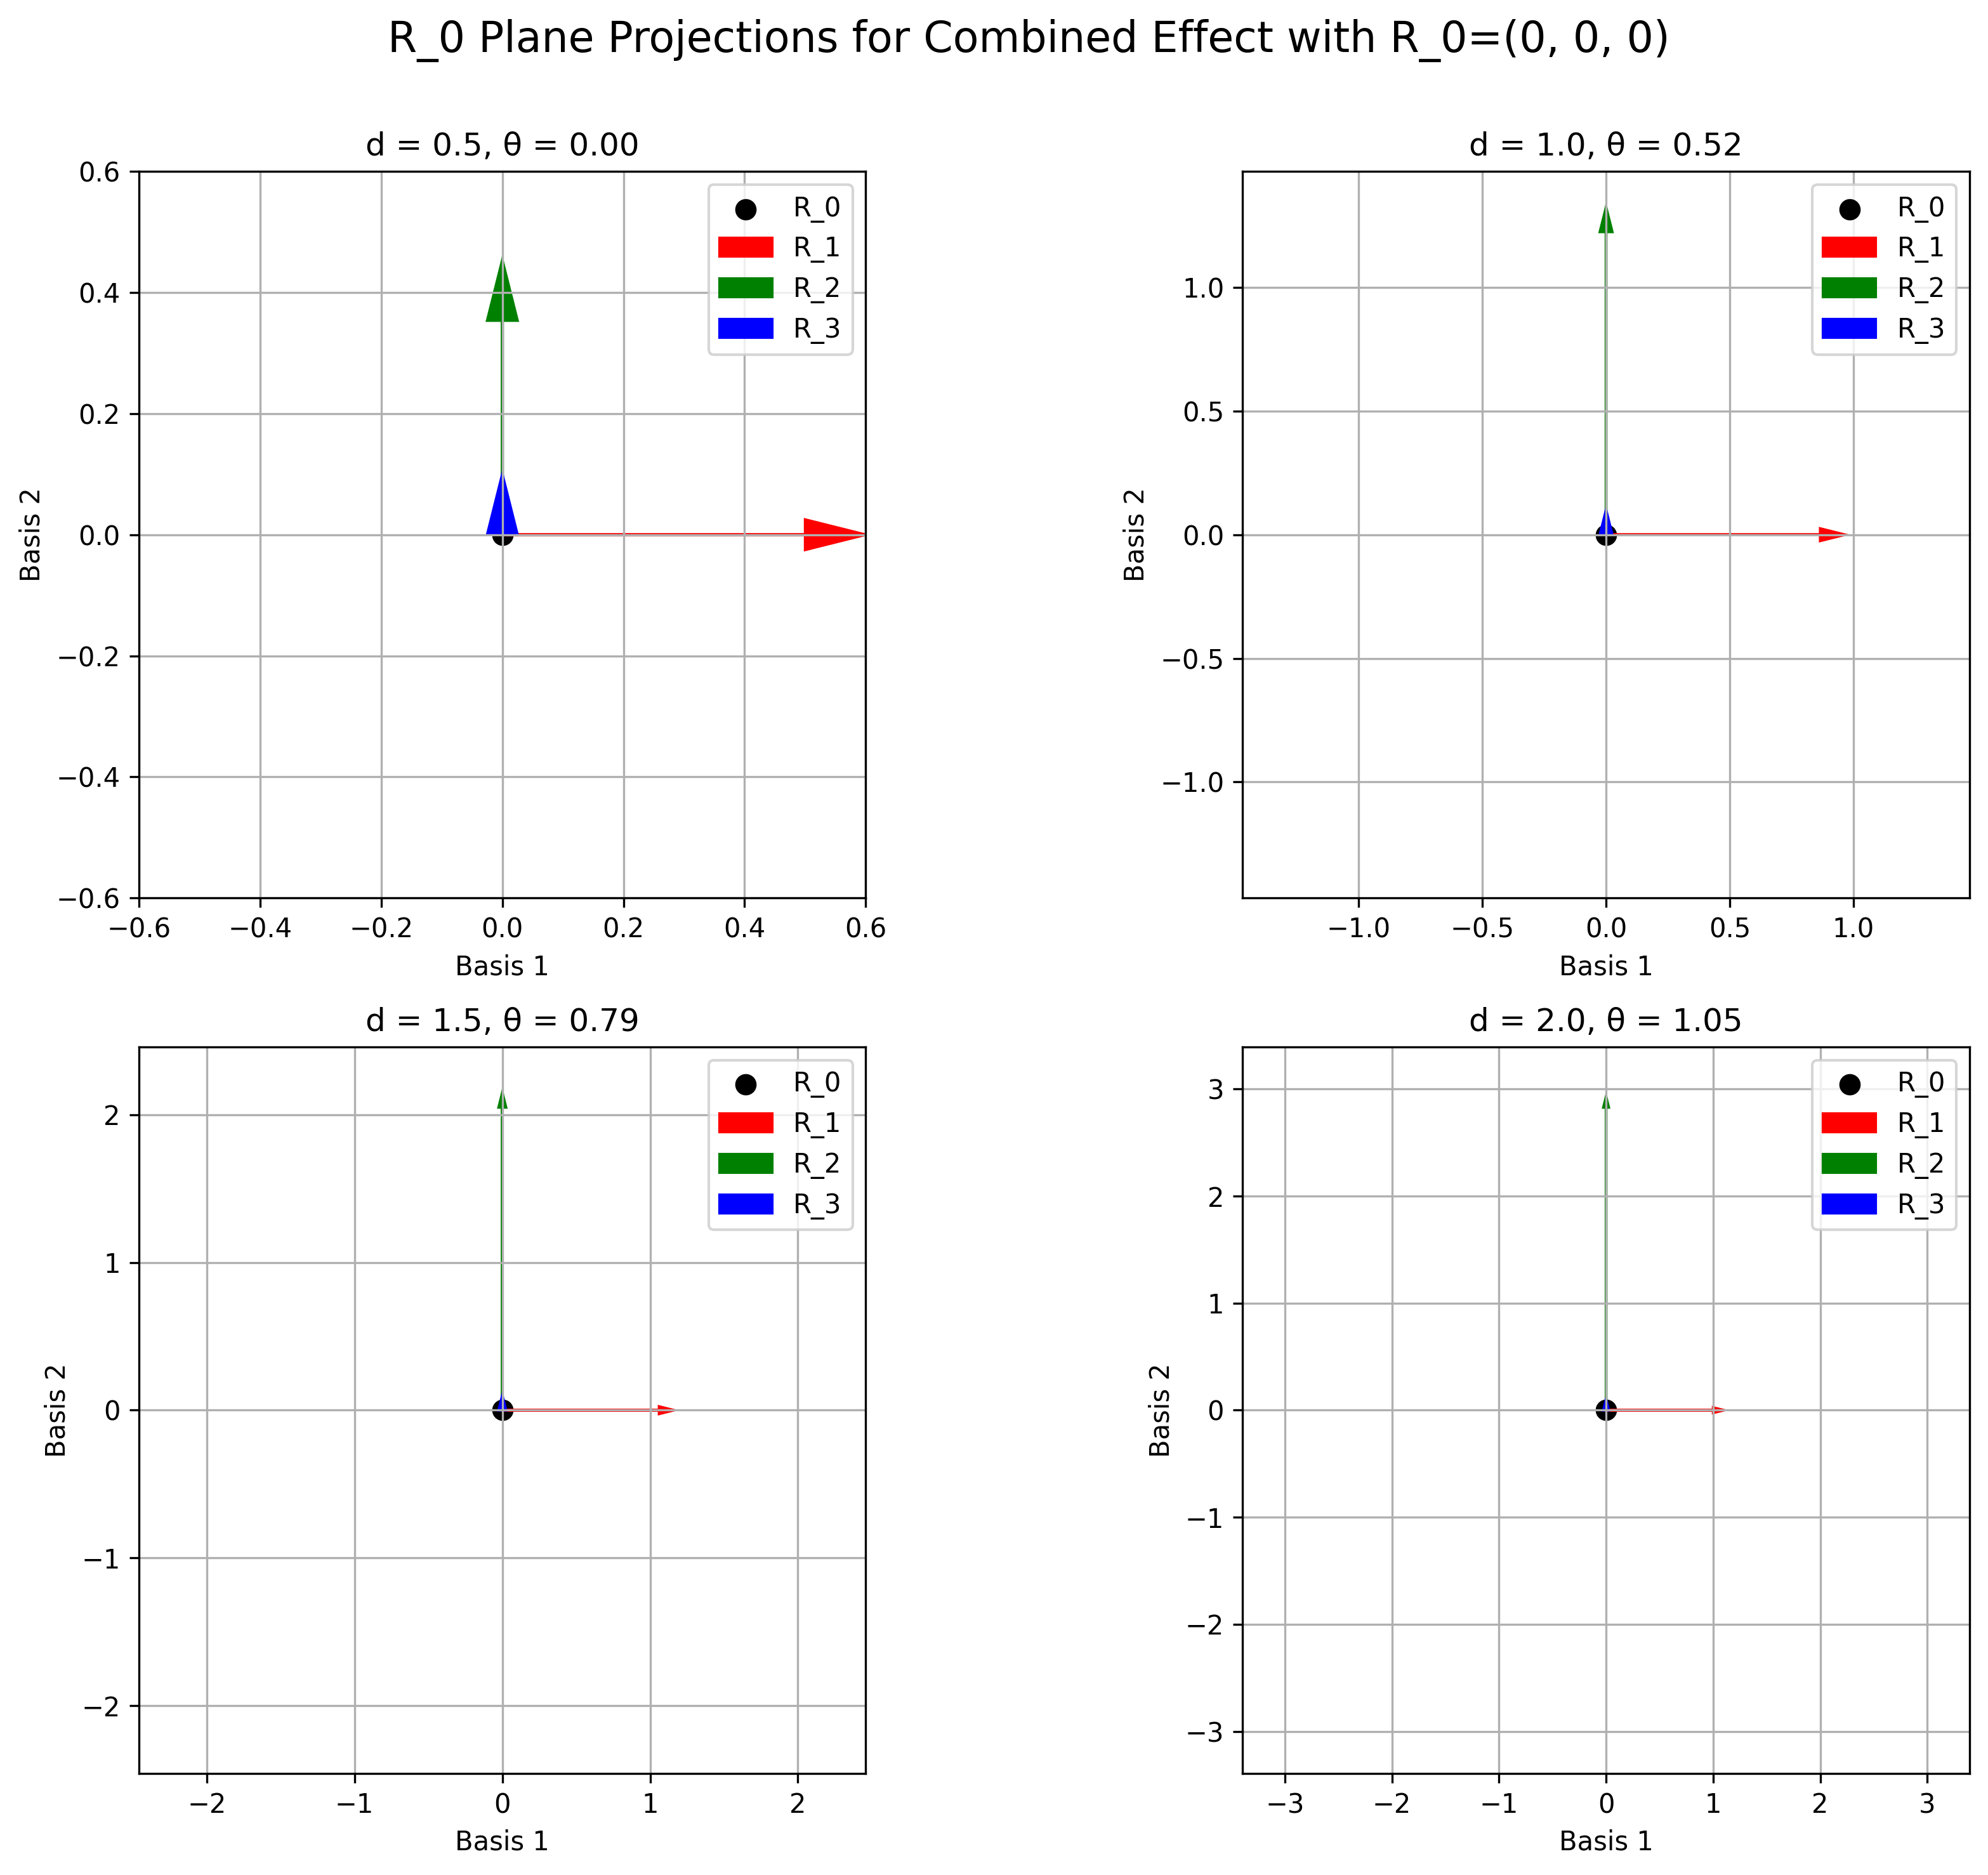
\includegraphics[width=0.8\textwidth]{figures/r0_projections_combined_effect_R0_0_0_0.png}
    \caption{Example of R0 plane projections}
    \label{fig:vis_r0_projections}
\end{figure}

\subsection{Implementation Details}

The visualization functions use Matplotlib to create the plots. The 3D visualization uses Matplotlib's \texttt{Axes3D} class, while the 2D visualizations use regular Matplotlib axes.

The vectors are plotted using Matplotlib's \texttt{quiver} function, which creates arrows from a starting point to an ending point. The origin point is plotted using Matplotlib's \texttt{scatter} function.

The colors of the vectors are assigned using Matplotlib's default color cycle, ensuring that each vector has a different color.

The legends are created using Matplotlib's \texttt{legend} function, with labels for each vector.

The plots are saved using Matplotlib's \texttt{savefig} function, which supports various file formats, including PNG, JPEG, and PDF.

\subsection{Visualization in the Command-line Interface}

The command-line interface provides options for controlling the visualization, including:

\begin{itemize}
    \item \texttt{--plot-type}: Specifies the type of plot, either "3d" or "2d".
    \item \texttt{--title}: Specifies the title of the plot.
    \item \texttt{--no-show}: Prevents the plot from being displayed interactively.
    \item \texttt{--save-path}: Specifies the path to save the plot.
\end{itemize}

These options allow users to customize the visualization without modifying the code.
